\documentclass[border=10pt]{standalone}
\usepackage[svgnames]{xcolor}
\usepackage{amsmath}
\usepackage{pgfplots}
\pgfplotsset{compat=newest}
\usepackage[sfdefault]{FiraSans}
\usepackage{FiraMono}
\renewcommand*\familydefault{\sfdefault}
\begin{document}
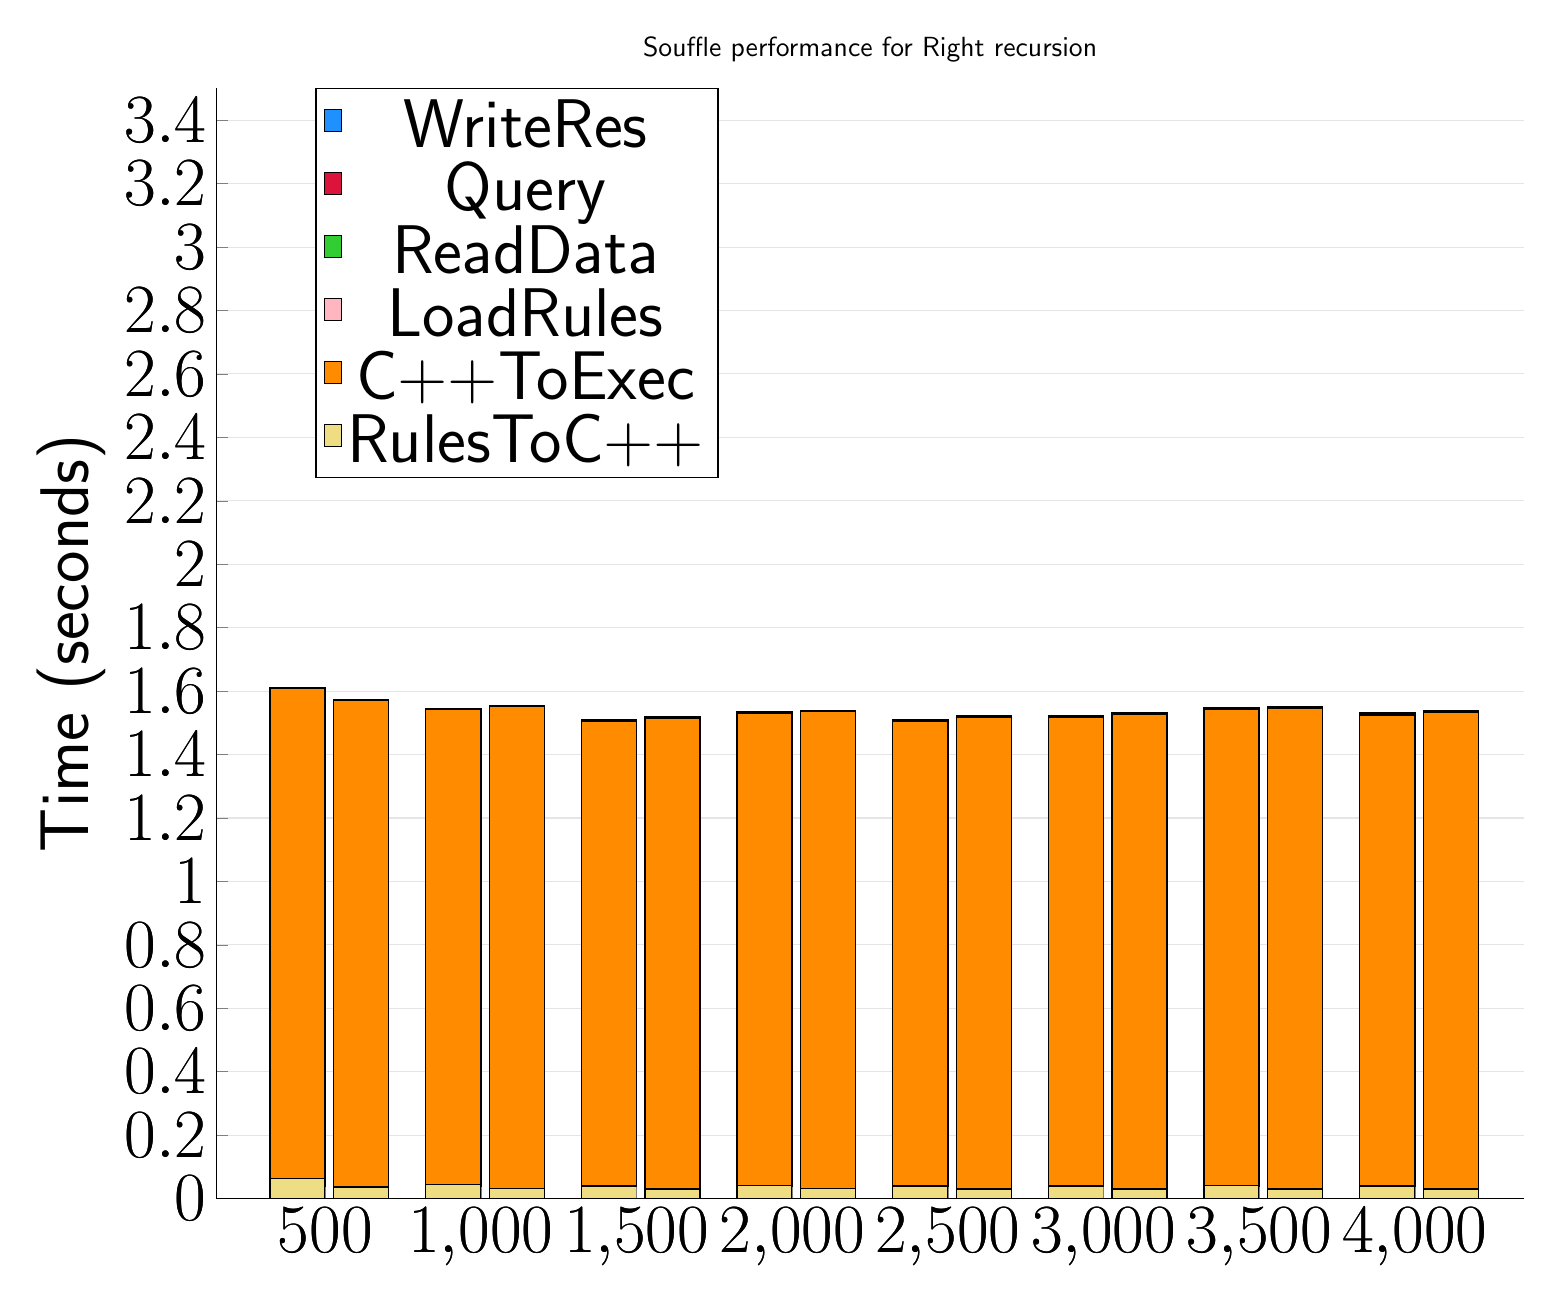
\begin{tikzpicture}
\begin{axis}[
   ybar stacked,
   title={Souffle performance for Right recursion},
   bar shift=-10pt,
   width=1.5\textwidth,
   bar width=0.7cm,
   ymajorgrids, tick align=inside,
   major grid style={draw=gray!20},
   xtick=data,
   ymin=0, ymax=3.5020000457763674,
   axis x line*=bottom,
   axis y line*=left,
   enlarge x limits=0.1,
   legend style={
       at={(0.23, 1)},
       anchor=north,
       legend columns=1,
       font=\Huge,
   },
   ylabel={Time (seconds)},
   label style={font=\Huge},
   tick label style={font=\Huge},
]
\addlegendimage{fill=DodgerBlue, draw=black, line width=0.2pt}
\addlegendentry{WriteRes}
\addlegendimage{fill=Crimson, draw=black, line width=0.2pt}
\addlegendentry{Query}
\addlegendimage{fill=LimeGreen, draw=black, line width=0.2pt}
\addlegendentry{ReadData}
\addlegendimage{fill=LightPink, draw=black, line width=0.2pt}
\addlegendentry{LoadRules}
\addlegendimage{fill=DarkOrange, draw=black, line width=0.2pt}
\addlegendentry{C++ToExec}
\addlegendimage{fill=LightGoldenrod, draw=black, line width=0.2pt}
\addlegendentry{RulesToC++}
\addplot +[fill=LightGoldenrod, draw=black, line width=0.5pt] coordinates {
    (500, 0.06299996376037598)
    (1000, 0.04499995708465576)
    (1500, 0.039999961853027344)
    (2000, 0.04200003147125244)
    (2500, 0.039999961853027344)
    (3000, 0.039999985694885255)
    (3500, 0.04200000762939453)
    (4000, 0.04000003337860107)
};
\addplot +[fill=DarkOrange, draw=black, line width=0.5pt] coordinates {
    (500, 1.547000002861023)
    (1000, 1.4970000028610229)
    (1500, 1.4659999847412108)
    (2000, 1.4890000104904175)
    (2500, 1.4640000343322754)
    (3000, 1.4760000228881835)
    (3500, 1.5009999752044678)
    (4000, 1.483999991416931)
};
\addplot +[fill=LightPink, draw=black, line width=0.5pt] coordinates {
    (500, 1.63e-05)
    (1000, 0.0)
    (1500, 1.0141600000000001e-05)
    (2000, 0.0)
    (2500, 0.0)
    (3000, 0.0)
    (3500, 0.0)
    (4000, 0.0)
};
\addplot +[fill=LimeGreen, draw=black, line width=0.5pt] coordinates {
    (500, 0.00044389989999999997)
    (1000, 0.00047105430000000004)
    (1500, 0.0007353751000000001)
    (2000, 0.0007057292)
    (2500, 0.0009181004)
    (3000, 0.0009840793999999998)
    (3500, 0.0010131805)
    (4000, 0.0011486072)
};
\addplot +[fill=Crimson, draw=black, line width=0.5pt] coordinates {
    (500, 0.0004943957)
    (1000, 0.0007922709)
    (1500, 0.0014499909999999999)
    (2000, 0.001774899)
    (2500, 0.0023284250000000007)
    (3000, 0.0029162829999999995)
    (3500, 0.003051801)
    (4000, 0.0034292240000000002)
};
\addplot +[fill=DodgerBlue, draw=black, line width=0.5pt] coordinates {
    (500, 0.0005668787)
    (1000, 0.0007658082)
    (1500, 0.001051808)
    (2000, 0.0011019654999999998)
    (2500, 0.0014065290000000001)
    (3000, 0.00171793)
    (3500, 0.0018360639999999997)
    (4000, 0.0020448739999999995)
};
\end{axis}
\begin{axis}[
   ybar stacked,
   bar shift=13pt,
   width=1.5\textwidth,
   bar width=0.7cm,
   ymajorgrids, tick align=inside,
   major grid style={draw=none},
   xtick=data,
   ymin=0, ymax=3.5020000457763674,
   axis x line*=none,
   axis y line*=none,
   enlarge x limits=0.1,
   label style={font=\Huge},
   tick label style={font=\Huge},
]
\addplot +[fill=LightGoldenrod, draw=black, line width=0.5pt] coordinates {
    (500, 0.036)
    (1000, 0.031000000000000007)
    (1500, 0.030000000000000006)
    (2000, 0.031000000000000007)
    (2500, 0.030000000000000006)
    (3000, 0.030000000000000006)
    (3500, 0.030000000000000006)
    (4000, 0.030000000000000006)
};
\addplot +[fill=DarkOrange, draw=black, line width=0.5pt] coordinates {
    (500, 1.535)
    (1000, 1.52)
    (1500, 1.485)
    (2000, 1.504)
    (2500, 1.487)
    (3000, 1.4969999999999999)
    (3500, 1.5160000000000002)
    (4000, 1.503)
};
\addplot +[fill=LightPink, draw=black, line width=0.5pt] coordinates {
    (500, 1.6100000000000002e-05)
    (1000, 0.0)
    (1500, 0.0)
    (2000, 1e-05)
    (2500, 0.0)
    (3000, 0.0)
    (3500, 0.0)
    (4000, 0.0)
};
\addplot +[fill=LimeGreen, draw=black, line width=0.5pt] coordinates {
    (500, 0.0004419)
    (1000, 0.0004555999999999999)
    (1500, 0.0006709000000000001)
    (2000, 0.0006914)
    (2500, 0.0008541)
    (3000, 0.0009691999999999999)
    (3500, 0.0009981)
    (4000, 0.0010842)
};
\addplot +[fill=Crimson, draw=black, line width=0.5pt] coordinates {
    (500, 0.0004941)
    (1000, 0.0007919000000000001)
    (1500, 0.0014496)
    (2000, 0.0017690999999999998)
    (2500, 0.0023275000000000006)
    (3000, 0.0029155000000000006)
    (3500, 0.0030510000000000003)
    (4000, 0.0034281)
};
\addplot +[fill=DodgerBlue, draw=black, line width=0.5pt] coordinates {
    (500, 0.0004798)
    (1000, 0.0006351)
    (1500, 0.0009605000000000001)
    (2000, 0.0011011)
    (2500, 0.0014053)
    (3000, 0.0017162)
    (3500, 0.0017322999999999998)
    (4000, 0.0019574)
};
\end{axis}
\end{tikzpicture}

\end{document}
